\documentclass[]{article}
\usepackage[english, ku, titlepage]{ku-frontpage}
\usepackage[acronym]{glossaries}

\makeglossaries
%opening
\assignment{Master Thesis}
\title{Investigation of Whole Grain Wheat and Barley Intake Biomarkers}
\author{Tu Hu}
%\subtitle{by UPLC-MS Based Metabolomics}
\advisor{Supervisor: Lars Ove Dragsted \& Gözde Gürdenz}
\date{Jun, 2019}
\usepackage[backend=biber,style=nature,%sorting=ynt
]{biblatex}
%\addbibresource{barley1.bib}
\addbibresource{barley.bib}
\usepackage{tabularx}
\usepackage{graphicx}

\begin{document}
\maketitle
%% abstract
\begin{abstract}
	This calls for an abstract.
\end{abstract}
%% table of content
\tableofcontents
\newpage
\newacronym{cvd}{CVD}{cardiovascular diseases}
\newacronym{tc}{TC}{Total Cholesterol}
\newacronym{ldlc}{LDL-C}{Low Density Lipoprotein Cholesterol}
\newacronym{hdlc}{HDL-C}{High Density Lipoprotein Cholesterol}
\newacronym{tg}{TG}{Triglycerides}
\newacronym{crp}{CRP}{C-Reactive Protein}
\newacronym{wbb}{WBB}{Whole Barley Bread}
\newacronym{wwb}{WWB}{Whole Wheat Bread}
\newacronym{bfis}{BFIs}{Biomarkers of Food Intake}
\newacronym{lc-ms}{LC-MS}{Liquid Chromatography-Mass Spectrometry}
\newacronym{gc-ms}{GC-MS}{Gas Chromatography-Mass Spectrometry}
\newacronym{nmr}{NMR}{Nuclear Magnetic Resonance Spectroscopy}
\newacronym{ms/ms}{MS/MS}{Tandem Mass Spectrometry}
\newacronym{tims-pasef}{TIMS-PASEF}{Trapped Ion Mobility Spectrometry with Parallel Accumulation Serial Fragmentation}
\newacronym{hmdb}{HMDB}{Human Metabolome Database}
\newacronym{gnps}{GNPS}{Global Nature Products Social Molecular Networking}
\newacronym{aw}{AW}{After Wheat}
\newacronym{ab}{AB}{After Barley}
\newacronym{bw}{BW}{Before Wheat}
\newacronym{bb}{BB}{Before Barley}
\newacronym{pca}{PCA}{Principle Component Analysis}
\newacronym{plsda}{PLSDA}{Partial Least Squares Discriminant Analysis}
\newacronym{pqn}{PQN}{Probabilistic Quotient Normalization}
\newacronym{vip}{VIP}{variable importance in projection}
\printglossaries
\newpage
\section{Preface}

%\input{barley.bib}

\section{Introduction}
%\subsection{R, Tidy Format and Data Wrangling}
%R is an open-source data analysis language.
%R is perfect for bioinformatics analysis.
%Tidy format is a term used in R describing a philosophy of storing data. Tidy format has the characteristics:
%\begin{itemize}
%	\item each variable is in its own column
%	\item each observation, or case, is in its own row
%\end{itemize}
%If data is stored in tidy form. Data scientists spend less time fighting with the tools and more time working on your analysis.




\newpage
\section{Materials and methods}
\subsection{A mini-systematic literature review of whole grain wheat and barley intake biomarkers}
A systematic literature review of whole grain wheat and barley intake biomarkers was conducted. This will prioritize future work on the identification of new potential biomarkers and on validating them.

The mini-review referred '8-step' Biomarker of Food Intake Reviews (BFIRev) Guidelines \cite{Pratico2018}.

%ISI Web of Science
\subsubsection{Designing the review for whole grain wheat and barley}
The \textbf{objective} of this review is to identify and evaluate reported biomarkers for dietary assessment of whole grain wheat and barley.

\subsubsection{Searching for relevant BFI research paper}
Keywords used: 
(barley) AND (biomarker* OR marker* OR metabolite* OR biokinetics OR biotransformation OR pharmacokinetics) AND (intake OR meal OR diet OR ingestion OR consumption OR eating OR food) AND 
(human* OR men OR women OR patient* OR volunteer* OR participant*) AND 
(trail* or experiment OR study) AND (urine OR plasma OR blood OR serum OR excretion OR hair OR toenail OR faeces OR faecal water)

(wheat) AND (biomarker* OR marker* OR metabolite* OR biokinetics OR biotransformation OR pharmacokinetics) AND (intake OR meal OR diet OR ingestion OR consumption OR eating OR food) AND 
(human* OR men OR women OR patient* OR volunteer* OR participant*) AND 
(trail* or experiment OR study) AND (urine OR plasma OR blood OR serum OR excretion OR hair OR toenail OR faeces OR faecal water) since 2008

\subsubsection{Selecting and screening papers for quality and relevance}
The title and abstract were readed in order to remove irrelevant literatures.

\subsubsection{Selection of candidate BFIs and data collection from the included records}

\subsubsection{Assessing quality of included papers on candidate BFIs}


\subsubsection{Evaluating the current overall status of BFIs for the food in question}


\subsubsection{Presenting data and results}


\subsubsection{Interpretation and conclusion}

\subsection{Software}
Several software packages were used for different purposes.

MATLAB R2018a (9.4.0.813654) coupled with PLS toolbox was used for data processing, modeling.

MZmine 2.31, an open source data processing software for \acrshort{lc-ms} and \acrshort{gc-ms}. 

MassLynx was used to check mass spectra.

DataBridge, an \acrshort{lc-ms} data file conversion program built-in MassLynx developed by Waters.

XCMS Online was used for uni-variable data analysis.


\subsection{Data-preprocessing}
Data-preprocessing consists x steps.

% Data convertion
First, data format was converted by DataBridge from '.raw' to '.cdf'. '.raw' was the format directly generated by Waters analytical platform. In order to be readable by MZmine, data was converted\footnote{N.B. Although in MZmine manual, '.raw' file is described as a compatible format, in practice some weird errors were generated when '.raw' format was input into MZmine.}.

% MZmine step
Then, the data was preprocessed by MZmine (2.31) following the steps: peak detection, deisotoping, alignment and gap filling.

Positive mode and negative mode were separately processed because of different noise level and in-source reaction. Blank samples were also excluded in pre-processing.

% result
In the end, the detected features, including information of mass to charge ratio (m/z), retention time (rt) and intensities were output as '.csv' files for further investigation.

%XCMS
%\subsection{Data conversion from MATLAB to R}
%'m2r.R'\footnote{codes were reposited on GitHub: https://github.com/tuhulab/bfi-wholegrain/blob/master/r/m2r.R} can convert a matlab dataset into R tidy form.

\subsection{Statistics}
\subsubsection{Paired t test}
Paired-t test and unpaired-t test were conducted on XCMS Online (xcmsonline.scripps.edu).

\subsection{PCA}
PCA was used for quality control and outlier detection.

\subsection{PLSDA modeling}
PLSDA modeling was used to select variables that have significant differences. 

\subsection{Literature search}
using qian's article as a reference


\section{Results}
\subsection{Mini-systematic literature review of whole grain wheat and barley intake biomarkers}
\subsubsection{search results in ISI Web of Science}

barley markers:47

wheat markers: 264

\subsection{Unpaired t-test of Negative Mode Urine Samples}
\begin{tabular}{c|c|c}
	hi | hi
\end{tabular}

\subsection{PLSDA modelling to select variables of plasma samples}
plsda modelling can not select any significant features to distinguish 
\section{Conclusions}
Limitation of LC-MS based metabolomics BFIs discovery: 
(1) instruments and their maintainance plus the analytical method development and optimization are expensive.
(2) it always involves clinical or human trail. it is expensive, time and energy consuming
(3) knowledge of researchers: chemistry, food science, nutritional science, human physiology, data analysis and programming is needed.

Metabolites are fluctuating.
 


\newpage
\section{Appendix}
\subsection{Chromatogram of Barley Flour}
\begin{figure}[h]
    \centering
    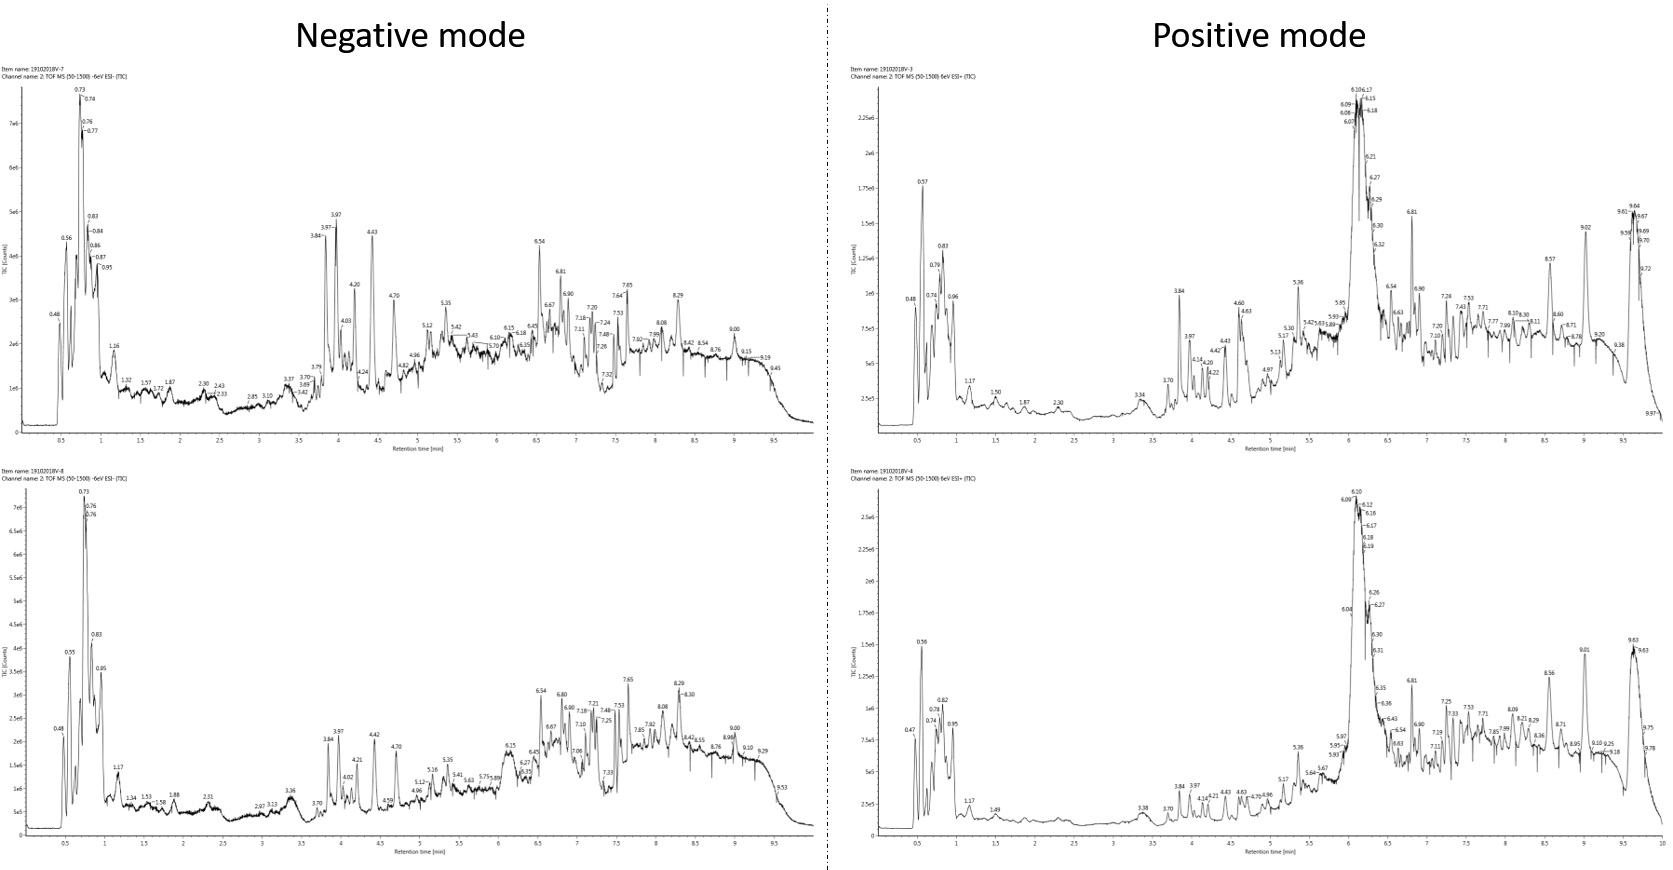
\includegraphics[scale=0.4]{images/chromatogram_barley_1.png}
    \caption{Chromatogram of Barley Flour (from top to the bottom: bran flour and endosperum flour)}
    \label{fig:chromatogram_barley}
\end{figure}

\clearpage
\subsection{\acrfull{ms/ms} spectra of phytosterols}
\acrshort{ms/ms} spectra of common phytosterols are shown in Figure \ref{fig:sterolmsms}, adapted from \cite{sterolms}
\begin{figure}[H]
    \centering
    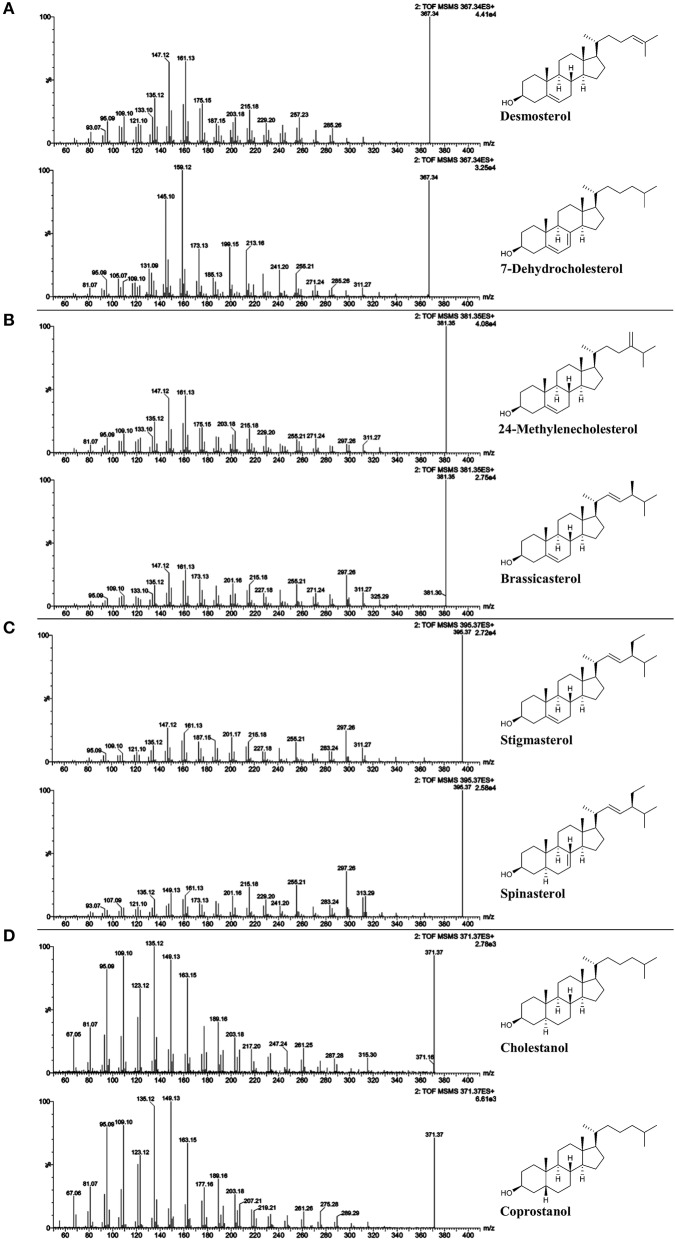
\includegraphics[scale=1]{images/sterolmsms.jpg}
    \caption{\acrshort{ms/ms} spectra of common phytosterols}
    \label{fig:sterolmsms}
\end{figure}

\end{document}
